\section{Reconstruction using SPINE}

When working with LArTPC detectors, fundamentally, all it returns is a series of voltages that have been read out to the  readout chips.
To get to a physics object from just a number of  voltages, a lot of work has to be done.
This process of converting from raw hits
\footnote{The individual voltages from a channell}
to physics objects is called reconstruction.

\begin{figure}[H]
  % 
  \centering
  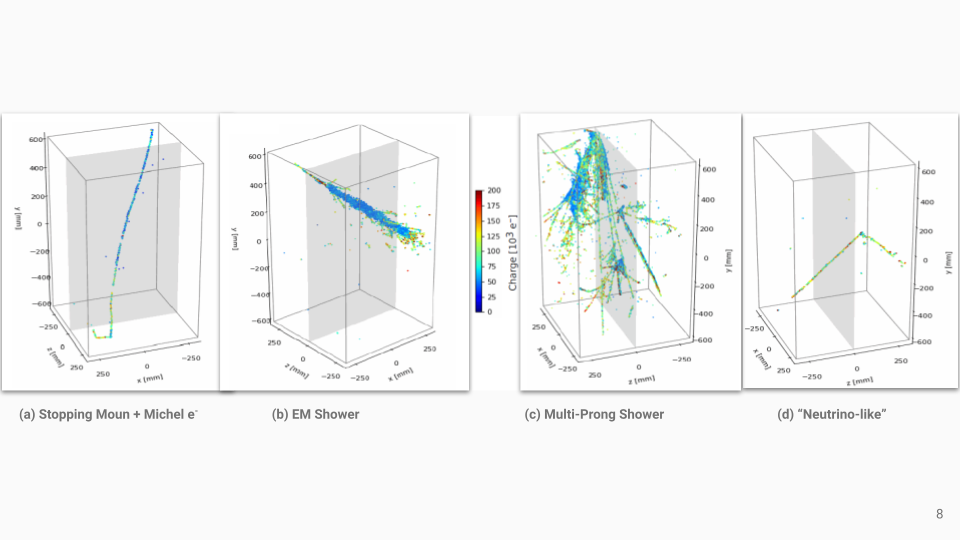
\includegraphics[width=120mm]{figures/mod0Events.png}
  \caption{Some reconstructed events from the module-0 prototype for the DUNE Near Detector}
  \label{mod0Event}
\end{figure}

There are a number of algorithims to do reconstruction of events, oftentimes with their own idiosyncracies, advantages and disadvantages.
The  Scalable Particle Imaging with Neural Embeddings (SPINE) package is one that uses machine learning to perform this reconstruction.

The SPINE  package is designed to work with LArTPC detectors with pixellated charge readout planes.
Traditionally, LArTPC detectors have used wire planes.
These generate a series of 2D pictures rather than  a native 3D image that is generated by a pixellated readout plane.
\footnote{There is an algorithm called  Cluster3D.
  This algorithm processes wire LArTPC data, which consists of three 2D images, to generate 3D points.
  However, this algorithm can introduce inefficiencies, resulting in ghost points—erroneous 3D points that shouldn't be there.}
The modules that are going to be part of the $2 \times 2$  prototype have pixellated planes, so we are good to use SPINE here.

We start with a root file produced either by simulation or with real LArTPC data.
That then gets run through LArCV  which is a C++ library to process LArTPC images.
LArCV processes the root files into what is called a sparse 3D input; just a list of coordinates that correspond to non-zero voxels (3d pixels)

After that, we can engage SPINE proper.

\begin{figure}[H]
  % https://github.com/DeepLearnPhysics/spine?tab=readme-ov-file  \centering
  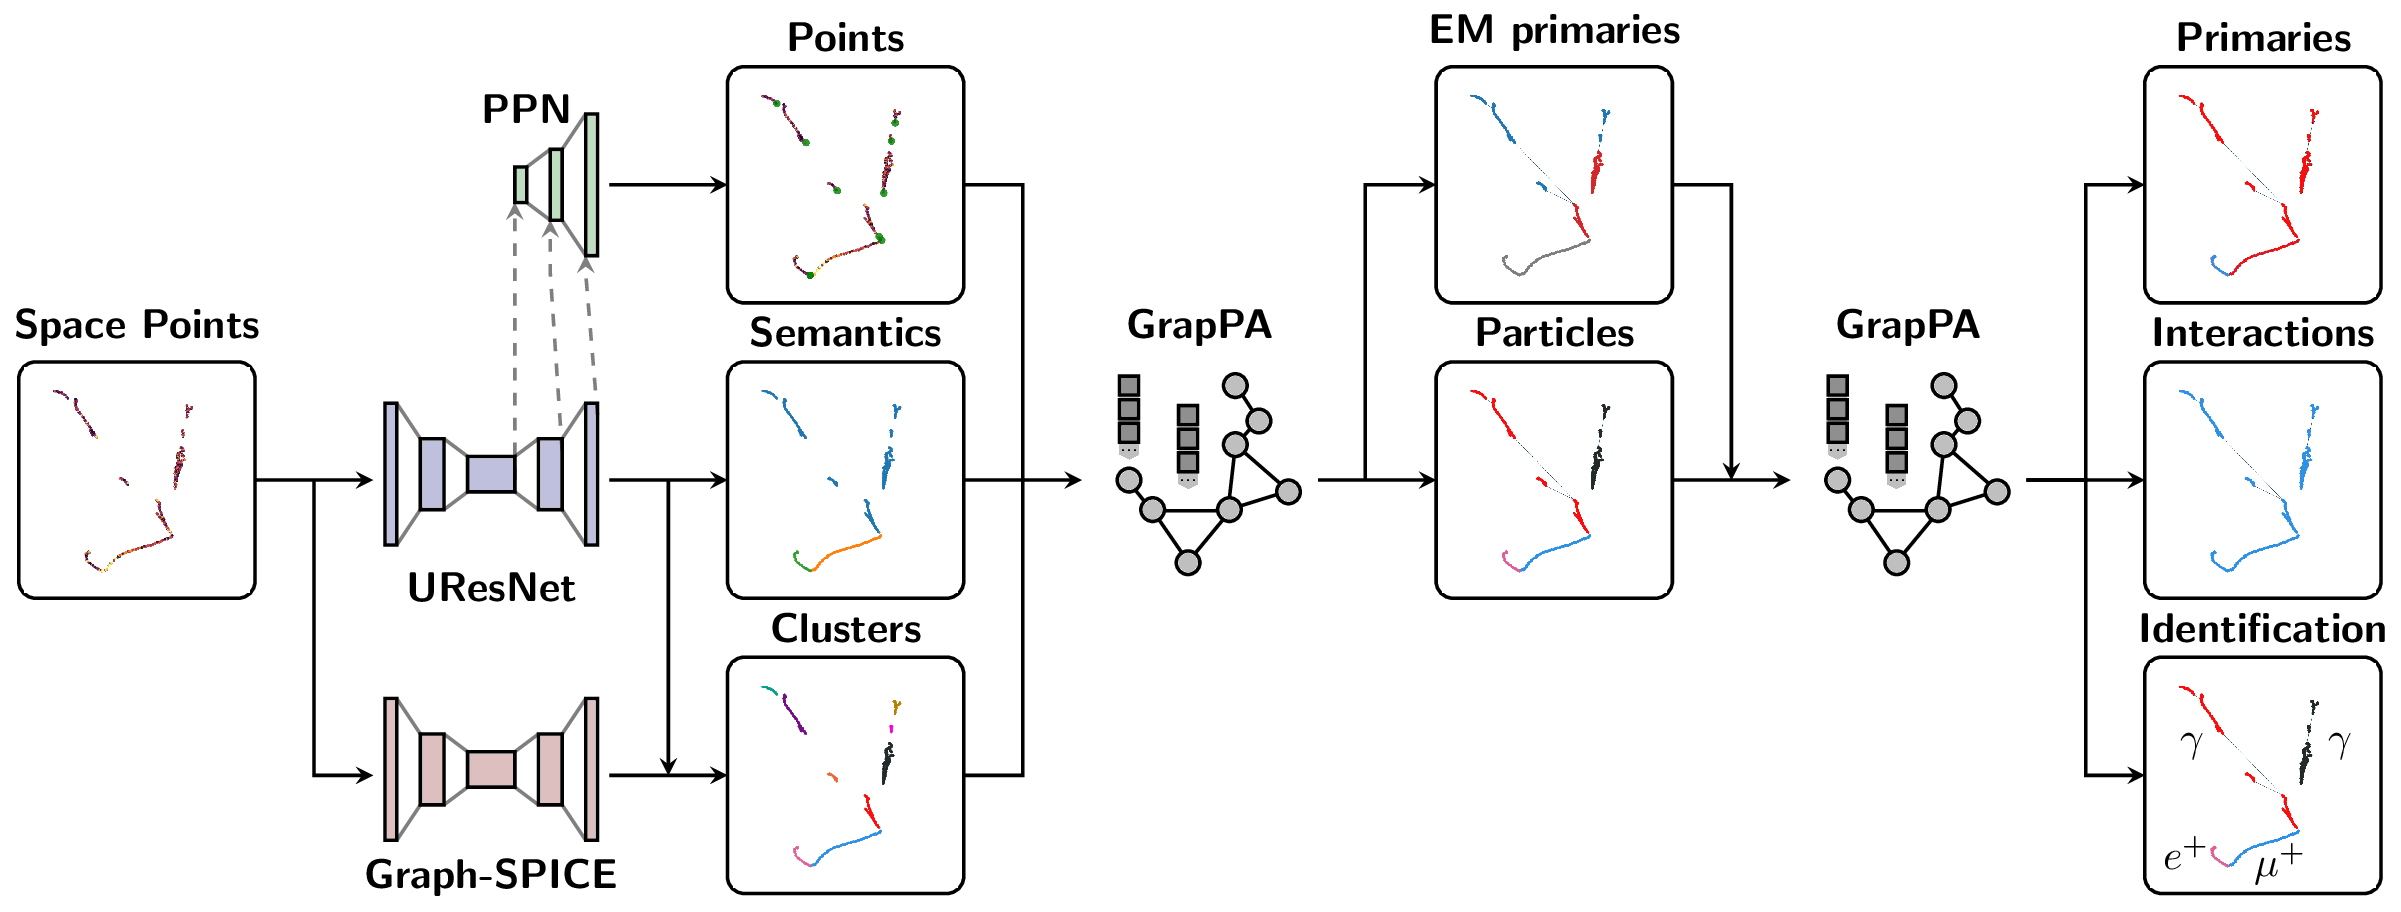
\includegraphics[width=120mm]{figures/spineSchematic.png}
  \caption{Overview of the SPINE schematic}
  \label{spineSchematic}
\end{figure}

SPINE consists of a number of machine learning models stitched together, workingin concert to get from raw hits to reconstructed outputs.
Let's break down each of the parts in turn.

